\chapter{Analysis}
\label{chap:analysis}
% TODO

\section{Methodology}
% TODO

\subsection{Performance gained by using multiple levels of detail}
\label{sec:analysis-mipmap}
The perception module (Section~\ref{sec:arch-perception}) of this work detects objects by matching their photos against camera images using the SIFT method (Section~\ref{sec:impl-sift}). Matching images against each other is a very performance intensive task. Let $I_1$ and $I_2$ be two images, $K_1$ and $K_2$ the corresponding sets of keypoints and $m_1 = |K_1|$ and $m_2 = |K_2|$ the maximum number of keypoints in each set. The maximum number of keypoints per set is limited by the size of the image: $m_1 <= |I_1|$ and $m_2 <= |I_2|$. Sample images are never larger than the camera images they are matched against (Section~\ref{sec:impl-db-limits}), therefore it is established that one image is at most as large as the other: $|I_1| <= |I_2|$. In conclusion, the complexity for the worst case is $O(m^2)$ with $m = m_1 = m_2$.

In order to be able to match multiple images in a sufficiently fast manner, $m$ is reduced by initially scaling down the images. The full sized images are only used if an object is detect in the scaled down version, to improve the projection from sample to camera image (Section~\ref{sec:impl-mipmap}). This technique highly increases performance for larger databases of sample images. \\

To review the actual benefit of this method, the performance of the system needs to be quantified. The speed of execution of a computer program can be expressed in frames per second (FPS), a standard measurement for performance in real-time applications. It denotes the number of images processed in one second, where, in this case, ``images'' means camera images and ``processed'' matched against the entire set of sample images.

The increase in speed becomes visible when average FPS are measured for both configurations - with downscaling and without - and plotted against each other. Comparable results can be obtained by defining standard situations to be used in both configurations. The performance of the system depends on two parameters: The amount of sample images in the database and the number of currently visible objects. Situations of interest are any combination of large, medium and small databases and no, one and multiple visible objects. In order not to distort the results, the same objects should be used in both configurations, as well as the same distance to the visible objects. \\

It can be expected, that the performance without visible objects is much higher with downscaling, because in this case this method definitely needs to match less keypoints. On the other hand, when using downscaling and objects are visible, they will trigger the use of larger images, causing the performance to drop. For smaller databases, the speed might drop even below the speed without downscaling: If, for example, only one object exists in the database and this object is visible, then the configuration with downscaling will need to match both sizes, the configuration without downscaling only the original size.


\subsection{Stability improvements through ``tracking'' findings from previous frames}
\label{sec:analysis-tracking}
Section~\ref{sec:impl-mipmap} details how the system tries to detect objects that were successfully recognized in the previous frame. This method is supposed to stabilize the perception, i.e. increase the chance to detect currently visible objects. \\

To measure the success of this rudimentary tracking method, a situation can be created where it is known which objects are currently visible. An ideal output of the system can be derived from the definition of this situation. Then, when running the system with and without tracking, its output can be compared with the ideal output to calculate how close both variants come. Dropped frames, i.e. frames where a visible object was not successfully recognized, can be visualized with a binary graph (the x-axis indicating frames and the y-axis indicating if a specific object was detected). A consistent graph would indicate a stable perception, a ``busy'' graph would indicate a lot of dropped frames. \\

Distant objects are more difficult to detect, because they appear smaller on the camera image and exhibit less distinctive features to be matched against a sample. Therefore it can be expected, that the amount of dropped frames increases with a higher distance to the object. In order to get comparable results, distance and angle between camera and object need to be the same for tests with and without tracking. Situations with both, close and far distances, need to be tested: The improvement in stability with tracking should get higher for far distances (the perception of close objects is pretty stable even without tracking).


\subsection{Decrease in false-positives through discarding concave projections}
Sometimes the SIFT method (Section~\ref{sec:impl-sift}) finds false matches that cause the detection of objects that are not currently visible. Because this work deals with rectangular objects only, many errors can be identified by projecting recognized objects onto the camera image and checking if its corners form a convex quadrangle and no two opposite sites intersect (see Section~\ref{sec:impl-2Dpose}). \\

Evaluating the ratio of discarded false positives could be done analogues to the evaluation of the tracking method (see Section~\ref{sec:analysis-tracking}): A situation is created where it is known which objects are currently visible, but \underline{not} visible objects would be compared with detected objects, in order to identify false positives. However, false positives cannot be enforced to come up, making it hard to get comparable results. Thus, experiences made during the testing phase of the system need to suffice. Debug outputs and the visualisation module provided evidence, that a lot less false positives got into the memory of the semantic map after employing the aforementioned method to drop them.


\subsection{Better 3D pose approximations by queueing multiple findings}
\label{sec:analysis-poses}
SIFT matches can contain a lot of noise and OpenNI laser sensors are not very accurate. Both are causes for distortion when calculating the 3D pose of an object. Therefore, the semantic map keeps multiple poses of one object, enabling it to calculate an average and cancel out the noise (as detailed in Section~\ref{sec:impl-queue}). \\

By placing a new object in front of the camera during runtime, the change of the 3D pose assigned to this object by the semantic map can be observed. The pose should change rapidly at first, then approach a stable state. To illustrate this behaviour, the output of the system can be turned into a graph, where the x-axis represents time and the y-axis one parameter of the pose (thus, the result would consist of 3 graphs displaying the position and 3 graphs displaying the direction vector).

If the position of an object is established, the pose calculated by the system can be compared to the real pose. Thereby the quality of the approximation of a pose can be evaluated as well. \\

It is expected, that the observed pose approaches a stable state for a static scene, but might change when introducing camera movement. The system can only estimate a pose, because the result of its calculations depend on the quality of the SIFT matches (see Section~\ref{sec:impl-sift}) and the depth image (the laser sensor produces better results for front-facing surfaces as opposed to surfaces rotated away from the camera). \\


% TODO
%\subsection{Less false-positives by removing unconfirmed objects}
%Although many false positives can be discarded early, some get through the filters, get published by the perception and end up in the semantic map. Others are correctly recognized but change their position afterwards. The semantic map tries to identify these cases by checking if objects are detected more than once. Otherwise they get removed again (described in Section~\ref{sec:impl-memo}). \\


\subsection{Relevance of objects suggested by the evaluation function}
Users who need a specific object can query the semantic map to find out it can remember seeing such an object before. If multiple objects of this type were seen before, the semantic map suggests where to look first, by evaluating all candidates based on spatial and temporal distance (Section~\ref{sec:impl-eval}). \\

To assess if the evaluation function employed by the semantic map suggests the best candidates, a scene with a representative range of objects of one type can created. Representative means that objects for all possible extreme cases should be included in this scene, i.e. any combination of close / far locations and short / long times since these objects where detected. Because dealing with long distances and time spans is difficult in the lab, the necessary objects can be inserted artificially into the system. \\

It is expected, that the evaluation function will primarily favour close objects, but prefer more recently seen objects to previously seen objects, because it weighs spatial distance higher than temporal distance.


\section{Experimentation}
% TODO

\subsection{Measuring performance with and without multiple levels of detail}
\label{sec:experiment-fps}
In order to quantify the performance gained by using a second level of detail, FPS (frames per second) were measured as outlined in Section~\ref{sec:analysis-mipmap}: The OpenNI camera was placed in a fixed position and the perception was executed both with and without using a second level of detail, logging the average achieved FPS. Then, more and more objects were placed in front of the camera, to observe how it affects the performance. Furthermore, in order to test how the system performs in with large databases, the experiment was conducted again after adding additional objects. \\

Specifically, the experiment was conducted with 0 to 4 objects, each with 10, 15, 20 and 26 objects, each with and without downscaling camera and sample images initially. This makes a total of 40 logged performance tests. Not all of the results are shown here, because it only made a difference \textit{if} an object was visible, not \textit{how many} objects were visible at once. The following charts present the average FPS measured in selected situations, illustrating the overall system performance and the difference when running with a second level of detail:

\begin{figure}[H]
  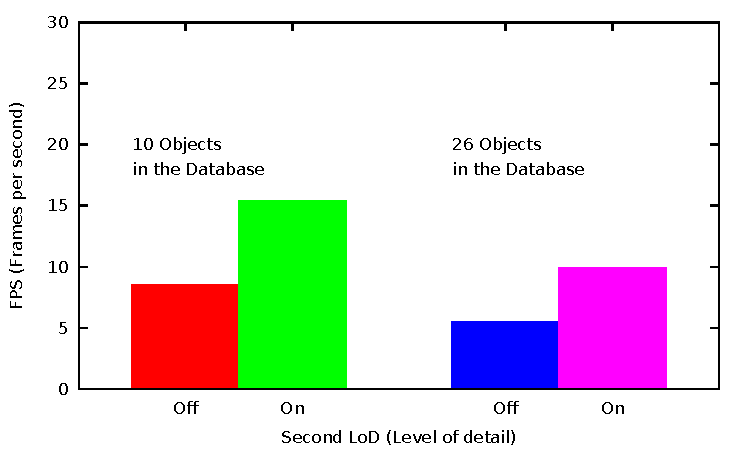
\includegraphics[width=1.0\textwidth]{images/fps-0-objects.pdf}
  \caption{FPS with 0 visible objects}
\end{figure}

\begin{figure}[H]
  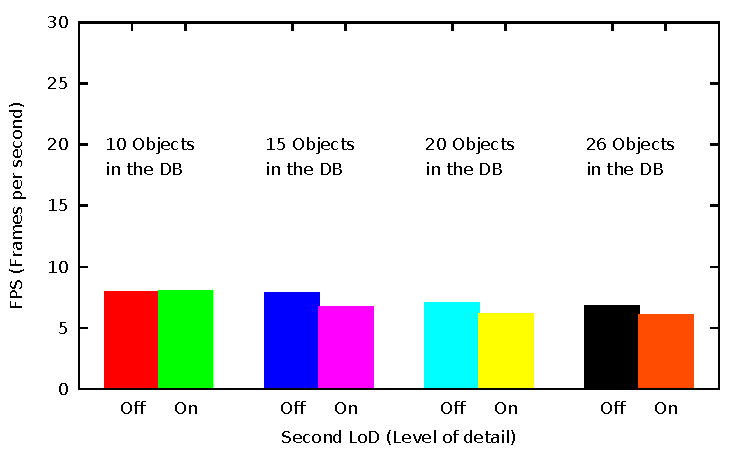
\includegraphics[width=1.0\textwidth]{images/fps-2-objects.pdf}
  \caption{FPS with 2 visible objects}
\end{figure}

In summary, the performance when running with a second level of detail was a lot faster without visible objects, but only slightly slower if objects were visible. Without a second level of detail, it did not make a difference if an object was visible, with a second level of detail the system was much faster if no objects were visible. Also, the performance got slightly slower with each object that was added to the database. The expectation expressed in Section~\ref{sec:analysis-mipmap} were met.


\subsection{Measuring the ratio of (un)successful object detections with and without tracking}
\label{sec:experiment-tracking}
The stability of the perception was assessed by setting up the OpenNI camera in a fixed position and putting an object known to the database in front of it. First, the object was placed close to the camera, then farther away, to find out how distance affects the stability. In order to measure the benefits of tracking objects found in the previous frame, the test was conducted with and without utilizing this method. Each frame, a boolean value was logged, denoting if the object was recognized during that frame or not.
\begin{figure}[H]
  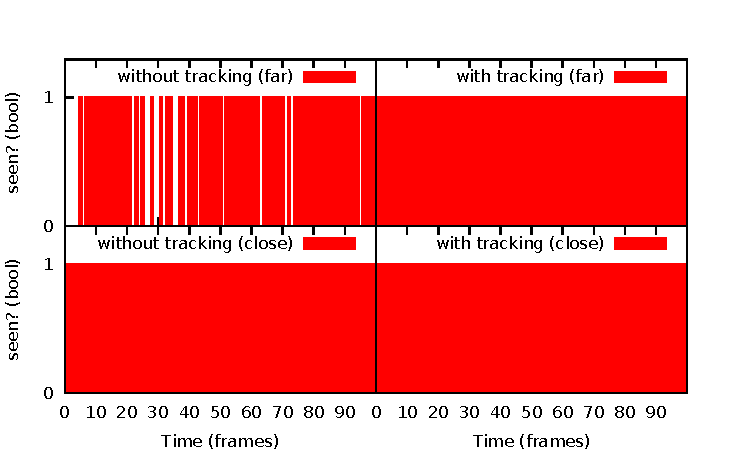
\includegraphics[width=1.0\textwidth]{images/perceptions.pdf}
  \caption{Successful objects detections with and without ``tracking''}
  \label{fig:analysis-perceptions}
\end{figure}

The results confirm the expectations from Section~\ref{sec:analysis-tracking}: Tracking does not help when recognizing objects close to the camera, because the perception already is pretty stable in this case. But it does improve the perception of objects farther away a lot. The gaps in the corresponding section in figure~\ref{fig:analysis-perceptions} illustrate that the object was not successfully recognized during many frames without tracking, when it was placed at a higher distance.


\subsection{Improvement and correctness of 3D Poses of recognized objects}
\label{sec:experiment-poses}
The 3D poses calculated for detected objects were evaluated in terms of correctness and stability, i.e. how close they match the real pose and how subsequent detections of the same objects improve the approximation (see Section~\ref{sec:impl-queue}).

To this end, a semi-static situation was created: The OpenNI camera was set up in a fixed position. After starting the system, an object was placed in front of it. Therefore, the pose calculated for this object could be observed from its inception until it did not change anymore. Then, the object was moved in front of the camera, to examine how long it takes for the system to adjust. \\

The following graphs illustrate the results of this experiment. The dotted lines denote the point in time when the object was moved. As expected, the values changed rapidly for newly detected objects and when the object moves, then converges to a pretty accurate approximation of the real object pose.

\begin{figure}[H]
  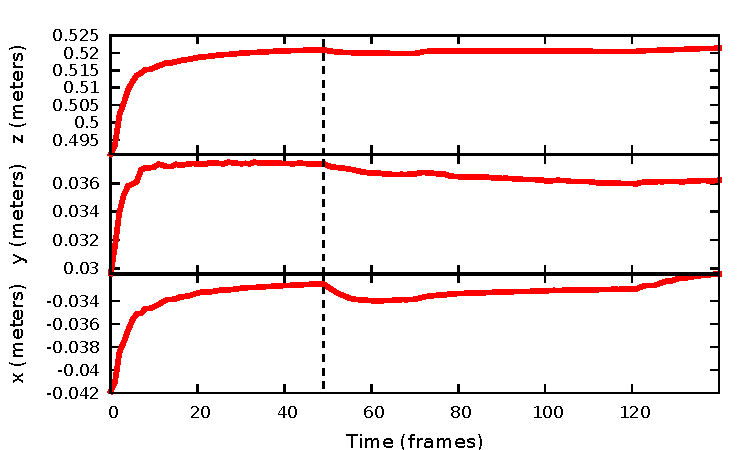
\includegraphics[width=1.0\textwidth]{images/3D-poses-position.pdf}
  \caption[3D poses position convergence]{3D pose position approximation. At around 50 frames, the position of the object changed slightly. Up until and after that point, the values converged to the real position.}
\end{figure}

\begin{figure}[H]
  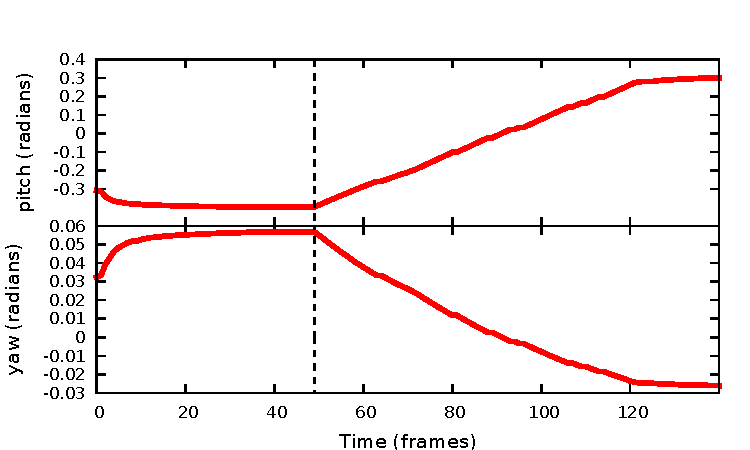
\includegraphics[width=1.0\textwidth]{images/3D-poses-orientation.pdf}
  \caption[3D poses orientation convergence]{3D pose orientation approximation. At around 50 frames, the orientation of the object changed. Up until and after that point, the values converged to the real orientation.}
\end{figure}

As described in Section~\ref{sec:analysis-poses}, the correctness of the approximated 3D pose of an object can be validated, if the real pose of the object used in the test situation is known. However, placing an object at exactly the right position and orientation is very hard. Instead, the visualisation module can be used to compare the calculated pose with the real pose. It publishes markers to the ROS visualisation tool rviz, to represent the objects memorised by the semantic map (see Section~\ref{sec:impl-viz}). rviz is able to draw a 3D model of the camera and depth images from the OpenNI camera, too. When overlaying this 3D model with the aforementioned markers, it can be observed how close the markers are placed to the actual objects they represent.

The results obtained with rviz can be seen in the screenshots above. The markers are placed right on top of the corresponding objects. The system reliably reached such a state in multiple tests with various objects placed at different positions and angles relative to the camera, when given a few seconds to adjust.


%TODO \subsection{Evaluation function}


\subsection{PR2}
\label{sec:experiment-pr2}
The previous experiments dealt with evaluating individual components of the proposed system, i.e. showing that the incorporated methods work correctly and what their benefits are. This section will focus on how these methods come together and perform in real-world applications. \\

\begin{wrapfigure}{r}{0.25\textwidth}
  \vspace{-10pt}
  \centering
  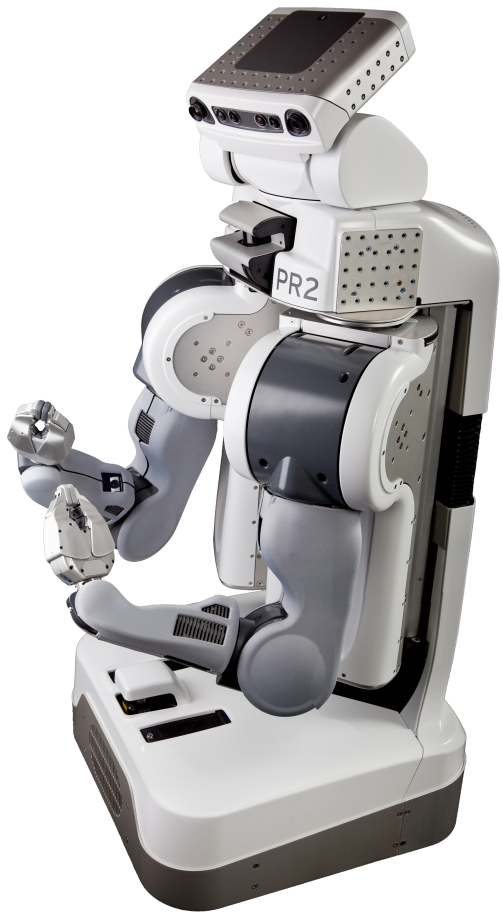
\includegraphics[width=0.23\textwidth]{images/pr2.png}
  \vspace{-10pt}
\end{wrapfigure}

For this experiment, a PR2 robot \todo{Reference} was used to run the system. The PR2 is a robot built by Willow Garage, the company that took over supporting OpenCV (an image manipulation library used in this work, see Section~\ref{sec:impl-opencv}), in 2008. Its software is written with ROS and is therefore compatible with the implementation of this work (see Section~\ref{sec:impl-ros}). It features a head-mounted Microsoft Kinect camera, which is a sufficient OpenNI camera, and a laser scanner at its base, used for localization (i.e. it knows the transformation from camera to map coordinates).

Various packaged goods that would be found at a store were placed on furniture all around the robot, in order to simulate a small supermarket scenario. The robot moved around its environment, looking at the objects and memorizing their locations. In the process, the state of the semantic map was observed with rviz. For this purpose, an existing 3D model of the environment for rviz was overlayed with the markers representing the objects memorized by the semantic map. \\

The resulting map was a quite accurate representation of the real world. When the robot was looking directly at objects, their poses were placed exactly at the right position. But, as expected, robot / camera movement introduced some light distortion and noise: Calculated positions appeared slightly shifted, and those that are misplaced farther than the length of the shorter side of the object cannot be resolved with the existing objects in the semantic map, so they end up getting added multiple times.


\section{Evaluation}
% TODO

\subsection*{Performance}
\label{sec:eval-performance}
The proposed system needs to be sufficiently fast, in order to be useful in real-world scenarios. It is supposed to enable a robot to recognize objects it passes while performing other tasks, as opposed to intentionally searching for them. The robot should not interrupt its current work and spend its time processing every interesting object it encounters.

The perception module is especially time-critical, because the OpenNI camera continuesly provides new images that need to be processed (the database and semantic map are more forgiving in terms of slight delays). The camera is capable of taking 30 images per second, and thereby determines a theoretical upper speed limit for the system. \\

In Section~\ref{sec:experiment-fps}, the performance of the system was measured in various different situations. As expected, the speed first and foremost depends on the number of sample images that need to be matched. But the results show, that the system is capable of real-time processing for reasonably sized databases of more than 20 objects.

Additionally, the aforementioned need to be able to keep the perception running while doing other work is addressed by the option to use scaled down images, until an interesting object comes into view (see Section~\ref{sec:analysis-mipmap}). The experiments demonstrate, that this method indeed saves a lot of processing power if no object is visible and is only marginally slower if an object is visible. The experiments also suggest, that the margin by which this method is slower during frames with visible object becomes smaller and smaller with each object added to the database. A break-even point could not quite be reached without adding such an amount of objects that would drastically slow down the system anyway, though. Still, that margin is always negligible in the context of the overall system performance.

\subsection*{Stability}
\label{sec:eval-stability}
Stability in the context of the perception means the amount of frames during which an object was recognized compared to the amount of frames during which that object was visible. The higher the ratio of successful detections, the better the approximation of the objects 3D pose. \\

The implementation includes a rudimentary tracking method, to ensure that the perception keeps detecting an object in subsequent frames, once it is recognized for the first time. The intention is to waste as little information as possible, because every successful detection helps improving the 3D pose.

Experiments have shown, that this method vastly increases the amount of successful detections of objects, especially if they are located farther away from the camera (Section~\ref{sec:experiment-tracking}). And because keypoints of successfully recognized objects are not investigated further (Section~\ref{sec:impl-multiple}), tracking can be applied without affecting the performance.

\subsection*{Correctness}
\label{sec:eval-correctness}
Correctness referes to how close the calculated 3D pose of an object is to reality. A pose consists of two parts: The position and the orientation.

The position is especially important, because it is the information required by a robot to find an object. As shown in the experiments (Section~\ref{sec:experiment-poses} and Section~\ref{sec:experiment-pr2}), the system can truthfully reproduce the objects location, but camera move can introduce a small offset. The cause for this distortion are slightly time-shifted transformations: The position calculated by the perception is correct, but the semantic map needs to transform it to a fixed coordinate system (see Section~\ref{sec:impl-memo}). The transformations provided by the tf package are never perfectly synchronized with images provided by the OpenNI camera, therefore transformations during camera movement will not be entirely correct. This is only a minor flaw though, because it does not compromise the end-result: The position is still very close to reality and will guide the robot in the right direction. Once it gets a closer look at the object, the perception will be able to calculate the correct position and resolve the misplacement.

The orientation is not mandatory for the proposed system to function, but it might be needed for certain tasks (if for example the robot needs to pick up the object). The tests show, that the implementation created in this work is capable of calculating a pretty accurate approximation of the orientation of an object. Thus, it does not only enable a robot to find objects more quickly, but it is also sufficient for 3D reconstruction in many pick-and-place scenarios.

